\chapter{Conexión local con BD externa} \label{cap:04BDEXt}

Aunque la base de datos de Eunomia permite satisfacer las necesidades ''demo'' de la herramienta, en la mayoría de las ocasiones el objetivo final de la implementación de ATLAS es realizar un estudio o investigación específica sobre una base de datos externa, propiedad del usuario o la organización que incopora la herramienta de análisis. Por tanto, es de gran interés presentar cómo establecer una conexión entre ATLAS Broadsea y una base de datos personalizada o propia. 

Esta conexión se realiza a través de la WebAPI de Broadsea (véase \ref{sec:01Postgre} ''Entorno PostgreSQL de Broadsea'') y, en la práctica, se puede realizar de dos formas distintas: 

\begin{itemize}
    \item \ref{sec:04ConfigManual} \textbf{Configuración manual}. Utiliza directamente el administrador de la base de datos . 
    \item \ref{sec:04ConfigAvanzada} \textbf{Configuración avanzada}. Utiliza los protocolos de seguridad de ATLAS y la webAPI .
\end{itemize}

El manual presenta ambas opciones aunque solo se seguirá en profundidad la configuración manual, ya que es la opción más sencilla y que los propios desarrolladores recomiendan para una implementación rápida \parencite{forumAddMSDB}. Por otra parte, por la naturaleza del entorno de instalación al que se enfoca este manual (véase \ref{sec:01IntroManual} ''Introducción al manual''), no es de interés activar el protocolo de seguridad de ATLAS , que debería ser la opción preferente para el despligue de la herramienta en organizaciones donde haya una necesaria diferenciación entre usuarios administradores con privilegios y usuarios sin privilegios. 

%Sin embargo, este caso no aplica puesto que la implementación se realiza para un grupo de investigadores en la que todos tienen los mismos privilegios de acceso.

\section{Configuración manual} \label{sec:04ConfigManual}

La configuración manual consiste en interactuar con la WebAPI directamente a través de pgAdmin para establecer la conexión con la base de datos externa. 

Esta implementación se describe de forma muy completa en la documentación correspondiente al repositorio de github de CDM Configuration \parencite{githubCDMConfig} y en los foros \parencite{forumAddMSDB}\parencite{forumBroadQuickStart}.

\subsection{Requisitos previos} \label{subsec:04RequisitosPrevios}

El único requisito que se necesita para poder integrar la base de datos externa con la WebAPI de ATLAS es que la base de datos externa esté estructurada según el CDM.

Esto implica una serie de características que se detallan en mayor profundidad en \ref{sec:01Postgre} ''Entorno PostgreSQL de Broadsea'', aunque se presentan otra vez a modo de resumen en este apartado:

\begin{enumerate}
    \item La base de datos debe estar conformada por los esquemas requeridos por el CDM \parencite{githubCDMConfig}, al menos: \code{cdm} y \code{results}
    \item Los datos y tablas de \code{cdm} deben estar normalizados a OMOP.
    \item No se requiere que haya un vocabulario explícitamente configurado para la base de datos externa pero debe haber un vocabulario configurado en Broadsea.
    \item Por último, no se requiere un estilo de base de datos concreto para la base de datos externa, puede ser Postgre o cualquier otro. 
    
\end{enumerate}

Para realizar esta implementación, según el fin educacional del manual, se utiliza la base de datos de synthea, que reúne todos estos requisitos. Para mayor información sobre la configuración de synthea consultar \ref{subsec:04OtrasBD}.

\subsection{Deployment} \label{subsec:04deployment}

La integración de la base de datos con la WebAPI es bastante sencilla, basta con configurar los parámetros correspondientes en el esquema \code{webapi} de la base de datos de Broadsea. Para ello se utiliza un listado de queries sql extraído de \parencite{githubCDMConfig}. También se puede descargar el archivo sql completo del repositorio del TFG \parencite{vallealonsodc}.

\begin{enumerate}
    \item En primer lugar, se debe añadir la nueva fuente en la tabla \code{sources} del esquema \code{webapi}. De este modo se registra la nueva fuente y el string jdbc que apunta hacia ella permitiendo la conexión. Para ello se puede utilizar la siguiente query:

\begin{lstlisting}[language=sql]
INSERT INTO webapi.source (source_id, source_name, source_key, source_connection, source_dialect) 
SELECT nextval('webapi.source_sequence'), 'My Cdm', 'MY_CDM', ' jdbc:postgresql://server:5432/cdm?user={user}&password={password}', 'postgresql';
\end{lstlisting}

    Donde:
    \begin{itemize}
        \item \code{source\_id}: Es el identificador de la fuente. Se asigna por defecto.
        \item \code{source\_name}: Es el nombre personalizado de la fuente.
        \item \code{source\_key}: Es la clave que utilizarán otras tablas para referirse a la fuente.
        \item \code{source\_connection}: Es el string de conexión jdbc, que debe seguir la estructura por defecto que se suigiere en la query. Si la
        \item \code{source\_dialect}: El dialecto que utiliza la base de datos. Por defecto sería postgresql.
    \end{itemize}

    Para el ejemplo de synthea, se aplica la siguiente query:

\begin{lstlisting}[language=sql]
INSERT INTO webapi.source (source_id, source_name, source_key, source_connection, source_dialect) 
SELECT nextval('webapi.source_sequence'), 'synthea1k', 'SYNTHEA1K', ' jdbc:postgresql://broadsea-atlasdb:5432/synthea1k?user=postgres&password=mypass', 'postgresql';
\end{lstlisting}

    Esto obtiene como resultado global:

\begin{figure}[H]
    \centering
    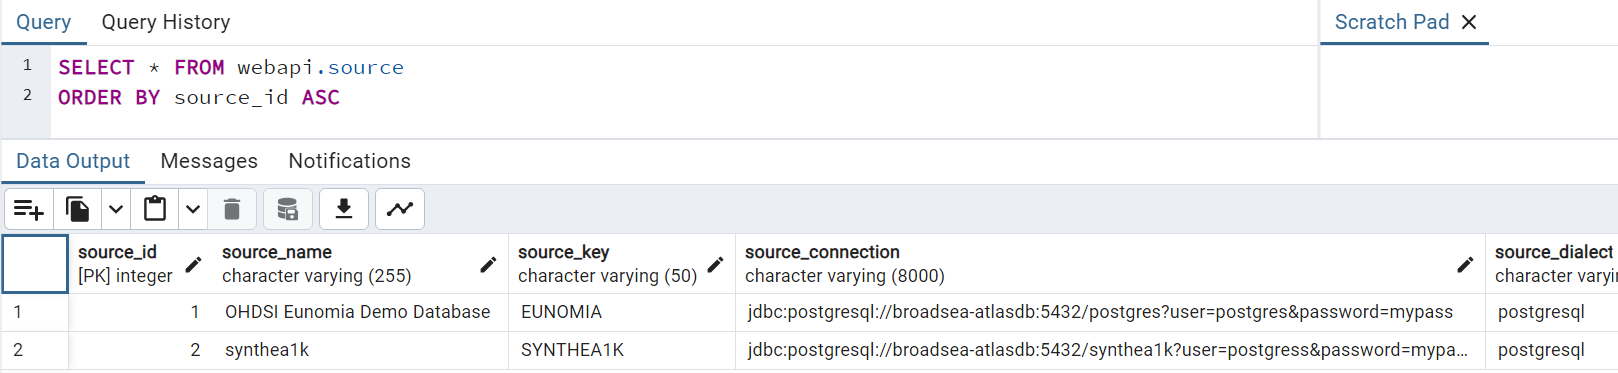
\includegraphics[width=0.90\textwidth]{figures/querySource.png}
    \caption{Captura de pantalla de las fuentes registradas en la tabla \code{sources}.}
    \label{fig:querySource}
\end{figure}
    

    \item En segundo lugar, y por último, se debe registrar cada esquema que utiliza la nueva fuente en la tabla \code{source\_daimon} del esquema \code{webapi}. Para ello se pueden utilizar las siguientes queries genéricas:

\begin{lstlisting}[language=sql]
INSERT INTO webapi.source_daimon (source_daimon_id, source_id, daimon_type, table_qualifier, priority) 
SELECT nextval('webapi.source_daimon_sequence'), source_id, 0, 'cdm', 0
FROM webapi.source
WHERE source_key = 'MY_CDM';

INSERT INTO webapi.source_daimon (source_daimon_id, source_id, daimon_type, table_qualifier, priority) 
SELECT nextval('webapi.source_daimon_sequence'), source_id, 1, 'vocab', 1
FROM webapi.source
WHERE source_key = 'MY_CDM';

INSERT INTO webapi.source_daimon (source_daimon_id, source_id, daimon_type, table_qualifier, priority) 
SELECT nextval('webapi.source_daimon_sequence'), source_id, 2, 'results', 1
FROM webapi.source
WHERE source_key = 'MY_CDM';

INSERT INTO webapi.source_daimon (source_daimon_id, source_id, daimon_type, table_qualifier, priority) 
SELECT nextval('webapi.source_daimon_sequence'), source_id, 5, 'temp', 0
FROM webapi.source
WHERE source_key = 'MY_CDM';
\end{lstlisting}

    Donde:
    \begin{itemize}
        \item \code{source\_daimon\_id}: Es el identificador del daimon. Se asigna por defecto.
        \item \code{source\_id}: Es el identificador de la nueva fuente, según el valor obtenido al registrar la fuente en la tabla \code{sources}.
        \item \code{daimon\_type}: Es el identificador que designa tipo de daimon que se está registrando, es decir, el tipo de esquema. Este identificador puede ser ''0'' para el esquema del \code{cdm}, ''1'' para el \code{vocab}, ''2'' para \code{results} y, opcionalmente, ''5'' para \code{temp}.
        \item \code{table\_qualifier}: Es el nombre concreto del esquema al que se está apuntando.
        \item \code{priority}: Es un valor entero mayor o menor que uno que sirve para distinguir cuál es la fuente prioritaria. Para el vocabulario y results, al menos debe haber un daimon con priority >= 1.  
    \end{itemize}

    Para la realización de esta implementación de ejemplo se ha seguido el ejemplo de synthea (véase \ref{subsec:04RequisitosPrevios} ''Requisitos previos''), que aplica las siguiente queries:

\begin{lstlisting}[language=sql]
INSERT INTO webapi.source_daimon (source_daimon_id, source_id, daimon_type, table_qualifier, priority) 
SELECT nextval('webapi.source_daimon_sequence'), source_id, 0, 'synthea', 0
FROM webapi.source
WHERE source_key = 'SYNTHEA1K';

INSERT INTO webapi.source_daimon (source_daimon_id, source_id, daimon_type, table_qualifier, priority) 
SELECT nextval('webapi.source_daimon_sequence'), 2, 1, 'cdm', 1
FROM webapi.source
WHERE source_key = 'SYNTHEA1K';

INSERT INTO webapi.source_daimon (source_daimon_id, source_id, daimon_type, table_qualifier, priority) 
SELECT nextval('webapi.source_daimon_sequence'), 2, 2, 'cdm_results', 0
FROM webapi.source
WHERE source_key = 'SYNTHEA1K';
\end{lstlisting}

    Esto se obtiene como resultado global:

\begin{figure}[H]
    \centering
    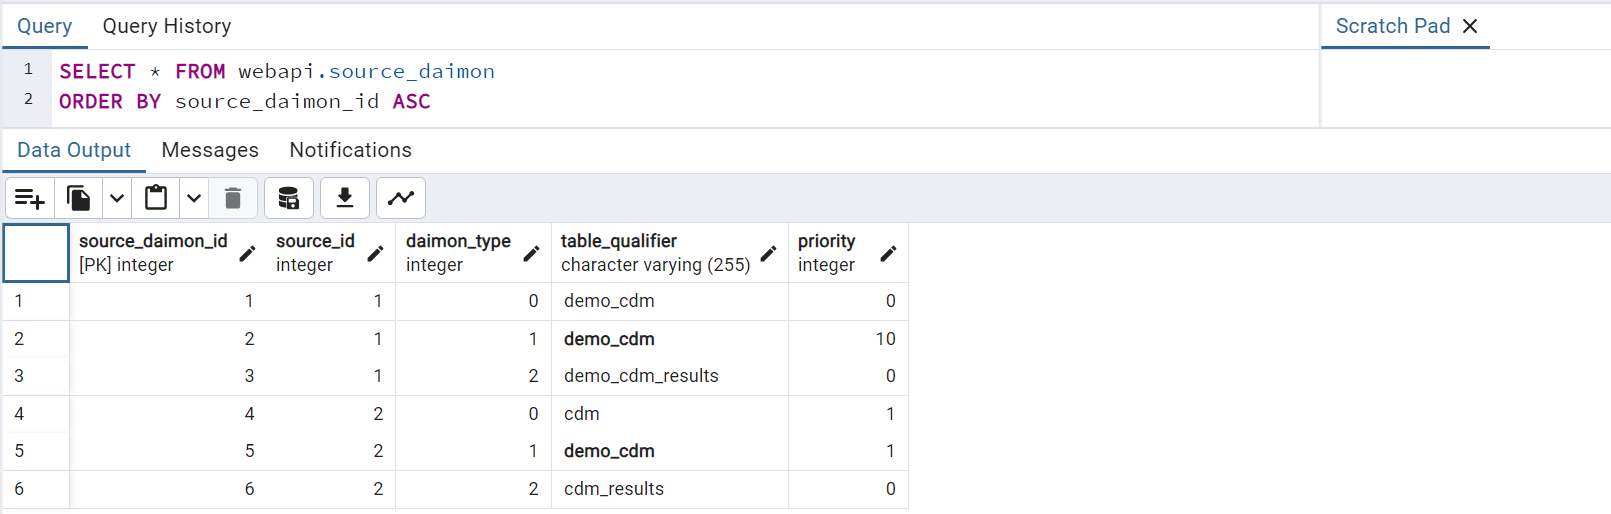
\includegraphics[width=0.90\textwidth]{figures/queryDaimon.png}
    \caption{Captura de pantalla de los daimon registrados en la tabla \code{source\_daimon}.}
    \label{fig:queryDaimon}
\end{figure}

    Observe que si se agrupase por \code{source\_id} hay dos fuentes distintas: (1) la fuente demo que viene preoconfigurada con Broadsea y (2) la fuente que se acaba de registrar.

\end{enumerate}

Así de sencillo, ya estaría registrada la nueva fuente, y establecida la conexión con la misma a través de la webAPI de Broadsea.

\subsection{Comprobación de conexión correcta} \label{subsec:04comprobacion}

Para comprobar que la conexión con la BD externa se ha realizado correctamente y se ha integrado correctamente con la WebAPI y con ATLAS se puede realizar dos estrategias:

\begin{enumerate}[label=\alph*]

    \item \textbf{Comprobación a través del navegador.} Acceder a la dirección \code{http://server/WebAPI/source/refresh} en el buscador del navegador y comprobar que aparece como primera fuente la base de datos de Eunomia y los esquemas que utiliza y, como segunda fuente, la base de datos añadida. El resultado debe ser similar al siguiente código:

\begin{lstlisting}[language=sh]
[{"sourceId":1,"sourceName":"OHDSI Eunomia Demo Database","sourceDialect":"postgresql","sourceKey":"EUNOMIA","daimons":[{"sourceDaimonId":1,"daimonType":"CDM","tableQualifier":"demo_cdm","priority":0},{"sourceDaimonId":3,"daimonType":"Results","tableQualifier":"demo_cdm_results","priority":0},{"sourceDaimonId":2,"daimonType":"Vocabulary","tableQualifier":"omop_vocab","priority":10}]},

{"sourceId":2,"sourceName":"synthea1k","sourceDialect":"postgresql","sourceKey":"SYNTHEA1K","daimons":[{"sourceDaimonId":4,"daimonType":"CDM","tableQualifier":"cdm\n","priority":1},{"sourceDaimonId":5,"daimonType":"Vocabulary","tableQualifier":"omop_vocab","priority":1},{"sourceDaimonId":6,"daimonType":"Results","tableQualifier":"cdm_results","priority":0}]}]
\end{lstlisting}

    \item \textbf{Comprobación a través de ATLAS.} Comprobar a través de la interfaz gráfica de ATLAS que aparece la nueva fuente, a través del menú deplegable del apartado \code{Data sources} o en el apartado \code{Configuration} de la herramienta.

\begin{figure}[H]
    \centering
    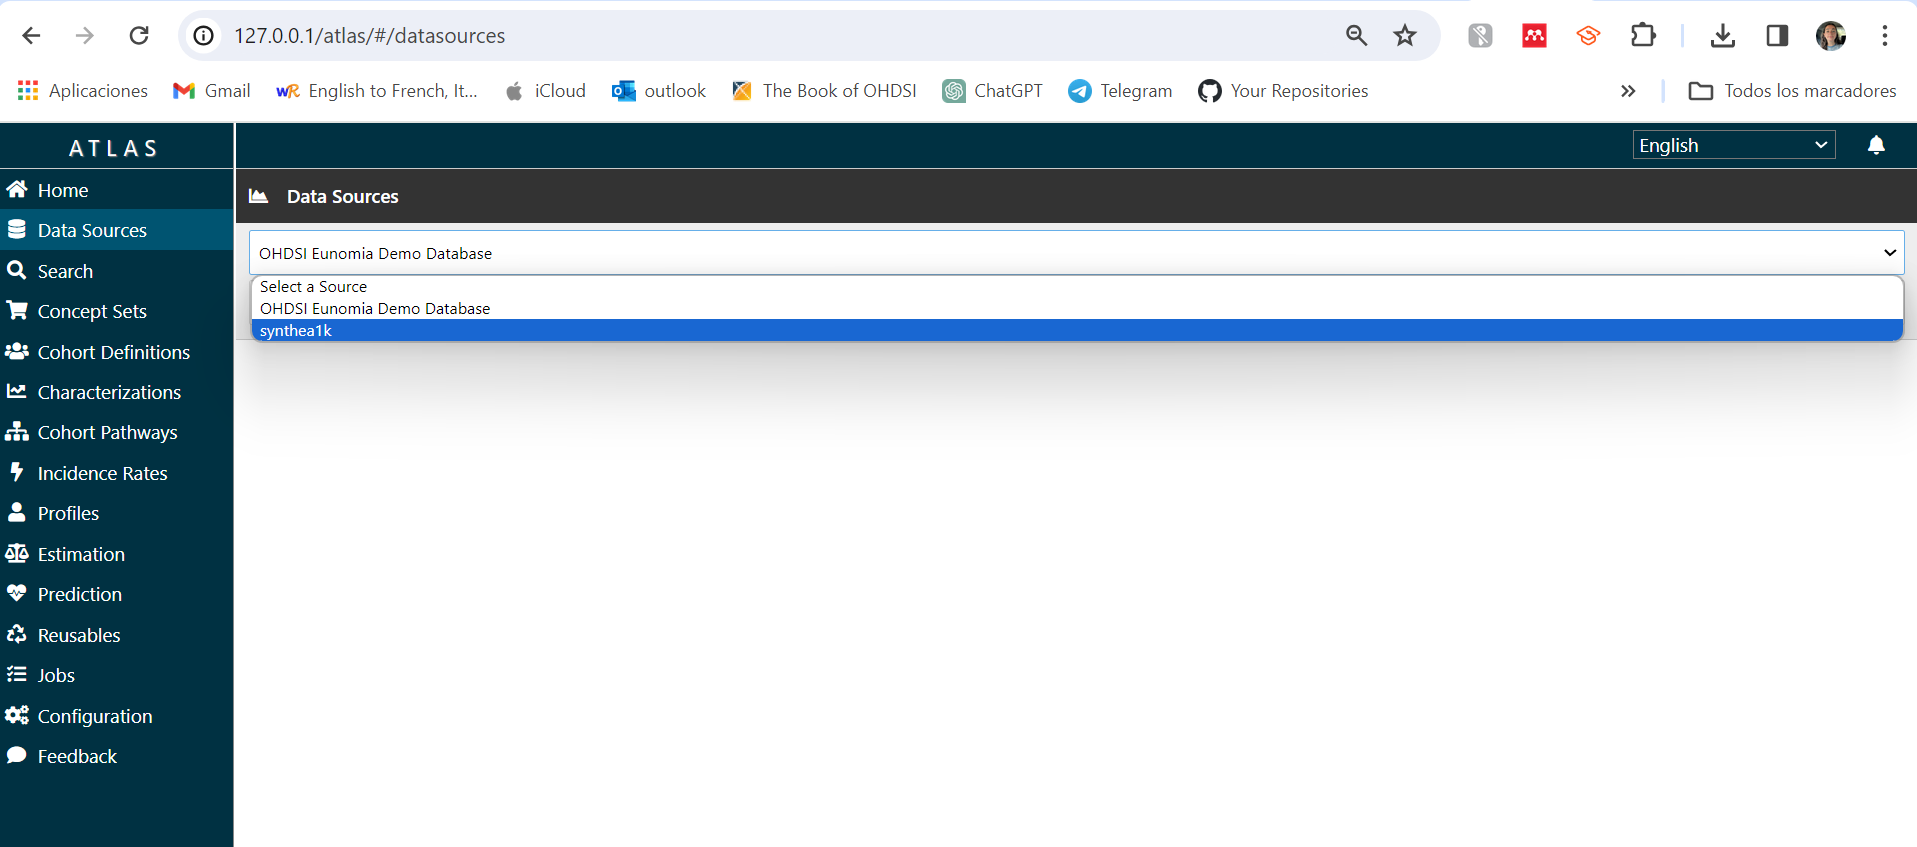
\includegraphics[width=0.90\textwidth]{figures/showDataSources.png}
    \caption{Captura de pantalla del menu \code{Data sources} de ATLAS Broadsea}
    \label{fig:showDataSources}
\end{figure}

\begin{figure}[H]
    \centering
    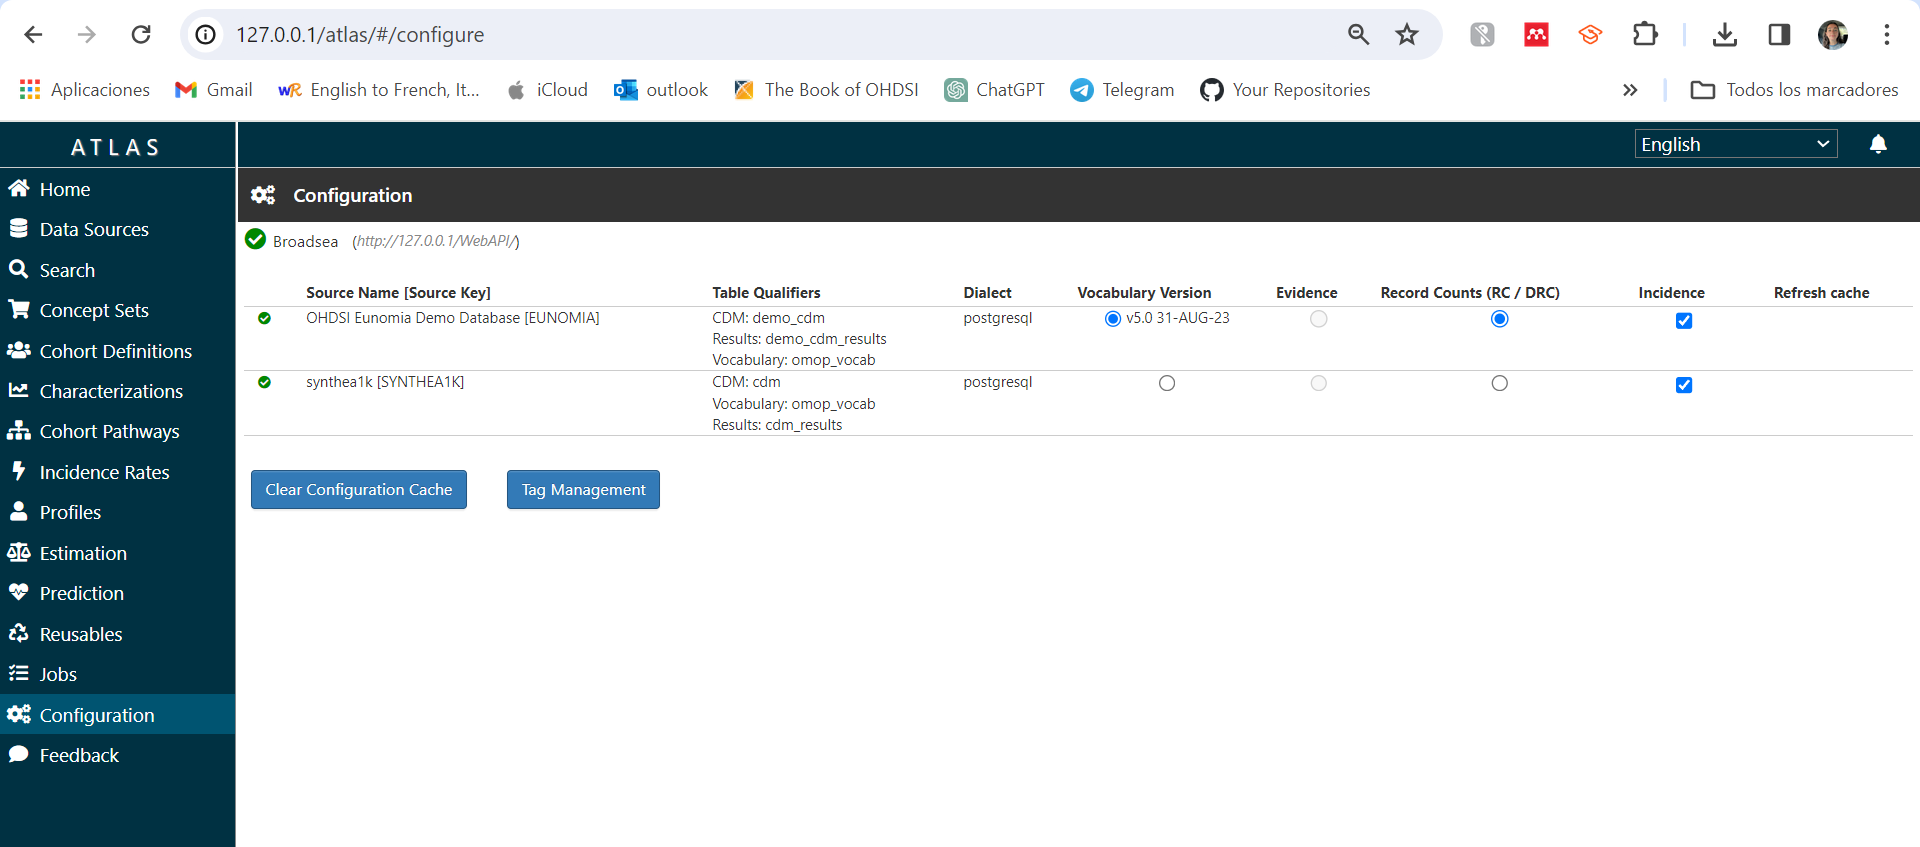
\includegraphics[width=0.90\textwidth]{figures/showConfiguration.png}
    \caption{Captura de pantalla del menu \code{Configuration} de ATLAS Broadsea}
    \label{fig:showConfiguration}
\end{figure}
\end{enumerate}

\subsection{Solución de posibles problemas}

%- Faltan esquemas no aparece

\subsubsection{Valores mal introducidos}

Problema: Al realizar las queries para introducir la base de datos la query no se ejecuta correctamente.

Motivo: No se reconoce el comando porque se ha introducido alguna palabra con error ortográfico.

Solución: Revisar las queries.

%\subsubsection{Error: Error loading report}

%Problema: Al querer generar un reporte de la base de datos recién introducida aparece dicho error.

%\begin{figure}[H]
%    \centering
%    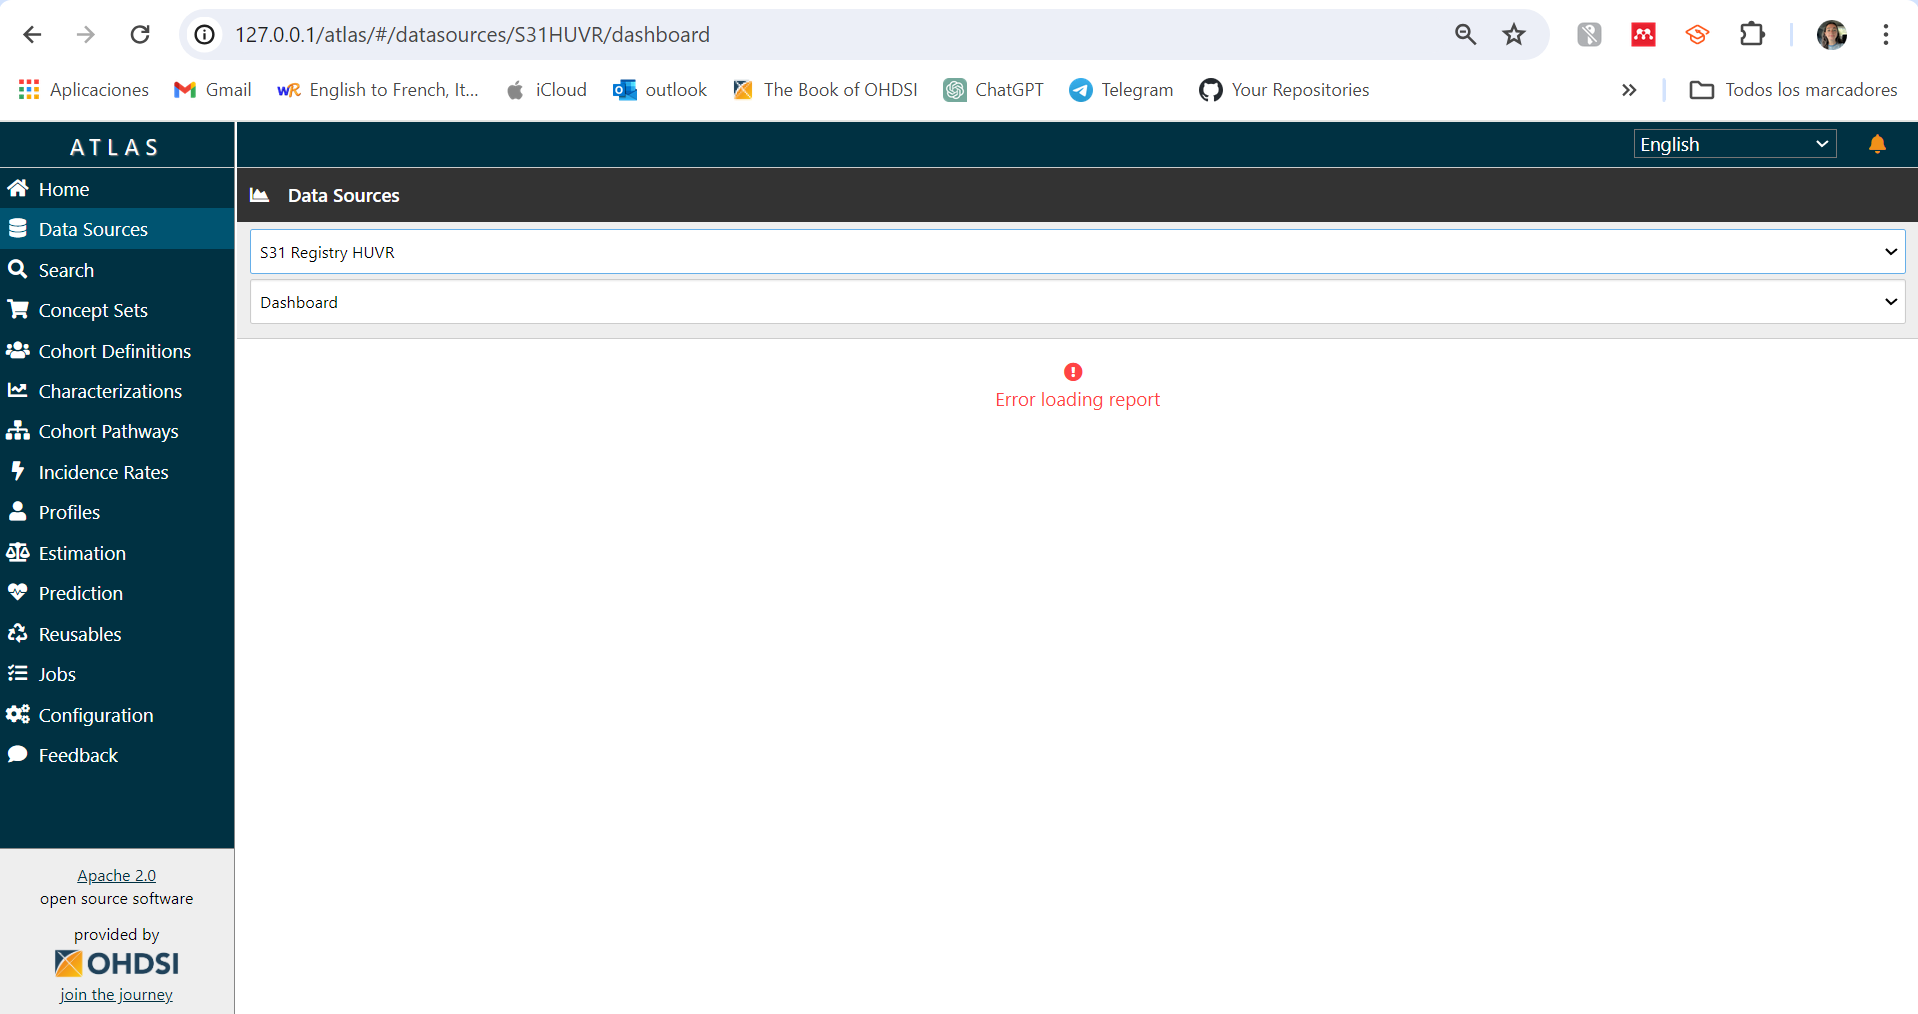
\includegraphics[width=0.90\textwidth]{figures/errorLoadingReport.png}
%    \caption{Captura de pantalla de error}
%    \label{fig:errorLoadingReport}
%\end{figure}

%Motivo: Para descubrir el motivo abrir el log de la WebAPI. En este caso el log 

%Solución: Hay que ejecutar ACHILLES sobre la base de datos antes de

\section{Otras configuraciones avanzadas} \label{sec:04ConfigAvanzada}

\subsection{Configurar la seguridad de Broadsea} \label{subsec:04Seguridad}

Otra forma de establecer conexiones con bases de datos externas es activando el protocolo de seguridad de ATLAS y de la WebAPI. Esta configuración posibilita la adición de fuentes a través de la interfaz gráfica de ATLAS, pues crea en el menú \code{Configuration} un nuevo boton para añadir fuentes intuitivamente. 

\begin{figure}[H]
    \centering
    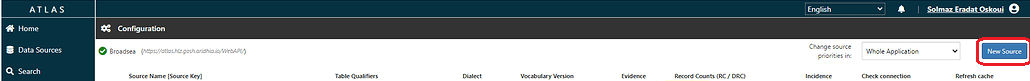
\includegraphics[width=0.90\textwidth]{figures/capNewSource.png}
    \caption{Imagen extraída de \parencite{forumAddMSDB} donde aparece el botón para añadir fuentes desde la interfaz gráfica de ATLAS}
    \label{fig:capNewSource}
\end{figure}

No obstante, esta forma tan aparentemente sencilla de conexión, verdaderamente se establece a través de protocolos complejos y configuraciones avanzadas de ATLAS y la WebAPI que resultan en grandes cantidades de problemas y errores. De hecho, en varias ocasiones los propios desarrolladores a través de los foros recomiendan su uso solo cuando sea extrictamente necesario \parencite{forumAddMSDB}\parencite{forumAddSecurityAtlas}.

Si bien la configuración es compleja, aporta, además de la facilidad de adición de fuentes mediante el botón en ATLAS, la posibilidad de distinguir entre distintos usuarios y roles con distintos permisos y privilegios, lo cual puede ser de gran interés en ciertos entornos u organizaciones.  La configuración de la seguridad de ATLAS empieza por la configuración de la seguridad de la WebAPI y ambas están descritas detalladamente en los correspondientes repositorios de Github \parencite{githubWASecurity}\parencite{githubATSecurity}. También hay un foro de gran interés en el que se describen aspectos de utilidad sobre la configuración de la seguridad en una organización \parencite{forumAddSecurityAtlas}.

\subsection{Descargar otras BD} \label{subsec:04OtrasBD}

Esta alternativa no es una configuración avanzada en sí misma pero si es una configuración opcional por lo que se encuadra en este marco. 

En principio, puede no ser de interés descargar otra base de datos demo si el objetivo del usuario es analizar con ATLAS su propia base de datos, pero puede ser de interés si tan solo se quiere probar el despliegue de la herramienta o su funcionalidad con una base de datos algo más extensa que la la base de datos de Eunomia, que es muy pequeña.

En este caso, precisamente para satisfacer esa necesidad, se ha descargado la base de datos de synthea.

\subsubsection{Synthea}

Realmente, synthea es un generador de datos sintéticos, no una base de datos por sí misma. Synthea permite construir una base de datos con parámetros configurables con información que no es real, pero podría serlo. La documentación de synthea se encuentra en su repositorio de github \parencite{githubSynthea} y en github pages \parencite{githubPagesSynthea}. Los datos de synthea no se crean por defecto estandarizados a OMOP pero OHDSI recoge también en un repositorio de github el rscript necesario para realizar el mapeo \parencite{githubETLSynthea}.

Para la realización de la configuración de la base de datos externa se ha creado manualmente una base de datos en Postgre, dentro del mismo servidor de Broadsea, con los esquemas \code{public}, \code{cdm} y \code{results}. 